\documentclass{webofc}
\usepackage{listings}
\usepackage{minted}
\usepackage{subfig}
\usepackage{hyperref}
\usepackage{graphicx}
\usepackage{subcaption}
\usepackage{tikz}

\usepackage[varg]{txfonts}   % Web of Conferences font

\newminted{cpp}{gobble=2,linenos=0, mathescape, numbersep=5pt, frame=lines, framesep=2mm, baselinestretch=1, fontsize=\footnotesize}
\newmintinline{cpp}{}

\newminted{bash}{gobble=2,linenos=0, mathescape, numbersep=5pt, frame=lines, framesep=2mm, baselinestretch=1, fontsize=\footnotesize}
\newmintinline{bash}{}

\usetikzlibrary{shadows, arrows, fit, positioning, matrix, shapes}
\usetikzlibrary{decorations.markings}

% Define colors
\definecolor{my_yellow}{RGB}{255, 253, 217}
\definecolor{my_orange}{RGB}{255, 127, 0}
\definecolor{my_lightblue}{RGB}{105, 186, 249}
\definecolor{my_purple}{RGB}{150, 154, 219}
\definecolor{my_green}{RGB}{90, 194, 160}

% Define block styles  
\tikzset {
  bigbox/.style = {draw, thick, fill=gray!10, rounded corners, rectangle},
  box/.style = {draw, thick, minimum height=0.8cm, minimum width=1.5cm, rounded corners, rectangle, fill=white, anchor=south},
  model/.style = {draw, thick, fill=white, text centered, minimum height=3em, minimum width=4em, rounded corners, drop shadow},
  user/.style = {draw, thick, ellipse, fill=white, text centered, minimum height=3em, minimum width=5em, drop shadow},
  line/.style = {->, thick, color=black, shorten <=2pt, shorten >=2pt, >=stealth'},
  plain/.style = {minimum width=1em},
  %\draw [line, ->] (m1.north) ++(-15pt,-1pt) arc [start angle=-140, end angle=-400, radius=20pt] node[midway] {$T_{M_1}$} ;
  % This works around an issue with node[midway] http://tex.stackexchange.com/questions/38763/how-to-place-a-node-in-the-middle-of-an-arc                
  arcnode/.style 2 args={
    decoration={
                 raise=#1,             
                 markings,   
                 mark=at position 0.5 with {\node[inner sep=0] {#2};}
            },
            postaction={decorate}
    }
}

% Define the layers to draw the diagram
\pgfdeclarelayer{background}
\pgfdeclarelayer{foreground}
\pgfsetlayers{background,main,foreground}

% Draw background
\newcommand{\background}[5]{%
  \begin{pgfonlayer}{background}
    % Left-top corner of the background rectangle
    \path (#1.west |- #2.north)+(-0.5,0.25) node (a1) {};
    % Right-bottom corner of the background rectanle
    \path (#3.east |- #4.south)+(+0.5,-0.25) node (a2) {};
    % Draw the background
    \path[rounded corners, draw=black!50, dashed, name=box]
      (a1) rectangle (a2);
    \path (a1 |- a2) -- (a2) node[midway,below] {\large\textit{#5}};
  \end{pgfonlayer}}

% Define a circled symbol command used throughout the thesis.
\newcommand*\circled[1]{\tikz[baseline=(char.base)]{
            \node[shape=circle,draw,inner sep=2pt] (char) {#1};}}
            
            %\input{./Figures/TikzCommon} % common tikz styles for the thesis


\begin{document}

\title{Optimizing Frameworks’ Performance Using C++ Modules Aware ROOT}

\author{\firstname{Yuka}
\lastname{Takahashi}\inst{1,2}
\fnsep\thanks{\email{yuka.takahashi@cern.ch}} \and
        \firstname{Vassil}
        \lastname{Vassilev}\inst{1}\fnsep\thanks
        {\email{vvasilev@cern.ch}}
        \firstname{Oksana}
        \lastname{Shadura}\inst{3}
        \fnsep\thanks{\email{oksana.shadura@cern.ch}}
        \firstname{Raphael}
        \lastname{Isemann}\inst{2,4}
        \fnsep\thanks{\email{isemann@student.chalmers.se}}
}

\institute{Princeton University \and CERN \and UNL \and Chalmers University of Technology}

\abstract{%
In this paper, we will present our results and challenges with C++ modules in ROOT. ROOT was extended with experimental support for using C++ modules during runtime, with aims to reduce its memory usage and improve its correctness. C++ Modules is a mechanism to boost {\it compilation} time.

However, it turns into runtime for ROOT as it's using Cling C++ {\it interpreter}. Especially, C++ Modules have a huge impact on the performance of experiments such as Atlas and CMS.

% Not sure if I should keep this two paragraph, looks a bit too long
The LLVM community advances its C++ Modules technology providing an io-efficient, on-disk code representation capable of reducing build times and peak memory usage. Significant amount of efforts were invested in teaching ROOT and its toolchain to operate with clang's implementation of the C++ Modules. Currently, C++ Modules files are used by: cling to avoid header re-parsing; rootcling to store io information in a cross-platform way; and ROOT's reflection layer to implement implicit and explicit runtime shared library loading.

ROOT builds and works with C++ Modules in its dictionary system showing promising performance. The conducted work paved our way for optimizing experiments' software stacks to achieve performance even beyond the observed in ROOT. The new technology adds three new requirements. First, every dictionary header needs to be parsable on its own. Secondly, it should not depend on outside macro definitions which can alter its content. Thirdly, all its direct or indirect includes should be also in a C++ Module. This talk shows the status of the C++ Modularization in ROOT and CMSSW. It argues for a bottom-up adoption approach and outlines a set of tools to aid the process. The authors share performance results and implementation experience gained when migrating CMSSW and its dependencies such as HepMC, Geant and boost.
% I copy pasted from CHEP proceeding, but it's not true because we didn't migrate to HepMC and Geant..
}
%
\maketitle
%
\section{Introduction}
\label{intro}

ROOT has several features which interact with libraries and require implicit header inclusion. This can be triggered by reading or writing data on disk, or user actions at the prompt. Often, the headers are immutable and re-parsing is redundant. C++ Modules are designed to minimize the re-parsing of the same header content by providing an efficient on-disk representation of C++ Code.

An implementation of the modules concepts exists in the LLVM frontend clang. Clang supports the Modules TS and hosts modules research and development work. The implementation encourages incremental, bottom-up adoption of the modules feature. Modules in Clang are designed to work for C, C++, ObjectiveC, ObjectiveC++ and Swift. Users can enable the modules feature without modifications in header files. The LLVM compiler allows users to specify module interfaces in dedicated file, called module maps files. A module map file expresses the mapping between a module file and a collection of header files. If the compiler finds such file in the include paths it automatically generates, imports and uses module files. The module map files can be mounted using the compiler’s virtual file system overlay mechanism to non-writable production library installations.

This paper is structured in six sections. First, we would like to explain a background and a motivation of this project. Next, we would like to dive into a detail of our implementation in ROOT. We'll show the result in section \ref{results}, and present our conclusion and future work.

\section{Background}
\label{background}

\subsection{Existing header parsing implementaion: Textual Include and PCH}
\label{tandpch}

\subsubsection{Textual Include}

In C/C++, the interface of a library is accessed by including the appropriate header files. This is a heritage from C, it's flexible but cause well-known problems, such as lacking of compile-time scalability and fragility.

\begin{itemize}
    \item \textbf{Compile-time scalability:}
    \#include is copying the contents to the includer's code, so the parser has to reparse the same common header files multiple times, which is expensive. As is illustrated in Figure \ref{fig:textual_include}, when the same header was included to different cxx file, it needs to be parsed again by a compiler the number of the time it was included. As shown in Listing \ref{list:expansion-of-textual-include}, the textual include can explode your object file.
    
\begin{figure}
\centering
    \begin{minipage}{.3\textwidth}
    \subfloat[] {\label{fig:perfBuildingROOT:a} \includegraphics[width=\textwidth]{tinc_image.png}}
    \end{minipage}
\caption{Image of re-parsing of the same header file}
\label{fig:textual_include}
\end{figure}

    \begin{listing}[h]
    \noindent
    \begin{minipage}[h]{.48\textwidth}
    \begin{cppcode*}{}
    #include "TVirtualPad.h"
    #include <vector>
    #include <set>

    int main(){...}
    \end{cppcode*}
    \end{minipage}\hfill
    \begin{minipage}[h]{.48\textwidth}
    \begin{cppcode*}
    # 286 "/usr/include/c++/v1/vector" 2 3
    namespace std { inline namespace __1 {
    template <bool> class __vector_base_common {
       __attribute__ ((__visibility__("hidden"),
       __always_inline__))
       __vector_base_common() {}
    ...
    # 394 "/usr/include/c++/v1/set" 3
    namespace std {inline namespace __1 {
    template <...> class set {
    public:
        typedef _Key key_type;

    int main() {...}
    \end{cppcode*}
    \end{minipage}
    \caption{Example of expansion of textual include}
    \label{list:expansion-of-textual-include}
\end{listing}

    \item \textbf{Fragility:} Textual includes are influenced by previously defined macros.
    For example, macro PI is \#defined in Rcpp library. Including this library while using local variable PI will end up in a redefinition error. Listing \ref{list:fragility} show how textual include can be fragile.
    
\begin{listing}[h]
    \noindent
    \begin{minipage}[h]{.48\textwidth}
    \begin{cppcode*}{}
    #define PI 3.14
    ...
    \end{cppcode*}
    \end{minipage}\hfill
    \begin{minipage}[h]{.48\textwidth}
    \begin{cppcode*}{}
    #include <header.h>
    ...
    double PI = 3.14;
    // => double 3.14 = 3.14;
    \end{cppcode*}
    \end{minipage}
    \caption{Fragility}
    \label{list:fragility}
\end{listing}

\end{itemize}

% PCH!!
\subsubsection{PCH}

The ROOT precompiled header (PCH) reduces the CPU and memory cost for ROOT’s most used libraries. The precompiled header technology is well-understood since decades. It is an efficient on-disk representation of the state of the compiler after parsing a set of headers. It can be loaded before starting the next instance to avoid doing redundant work. At build time, rootcling (ROOT’s dictionary generator) creates such PCH file which is attached at ROOT startup time. It's major drawback is the fact that if third-party users want to include their libraries, they have to recompile it every time there is a change. Figure \ref{fig:pchandpcm} demonstrates the difference of pch and pcm.

\begin{figure}[!h]
  \centering
  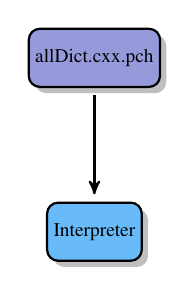
\begin{tikzpicture}[outer sep=0.05cm, node distance=0.8cm, scale=0.7, transform shape]
        
    \node[model, fill=my_purple, name=pch] (pch) {allDict.cxx.pch};
    \node[model, fill=my_lightblue, name=interpreter, below=2cm of pch] (interpreter) {Interpreter};

    \draw[line, ->] (pch.south) -- (interpreter);

  \end{tikzpicture}
  \hfill
  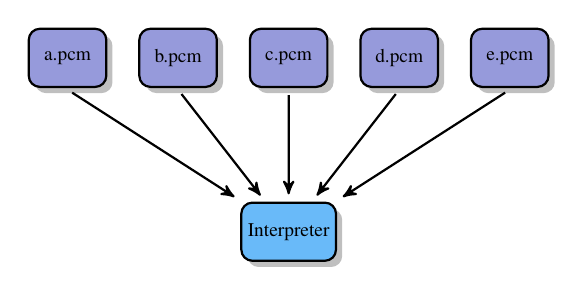
\begin{tikzpicture}[outer sep=0.05cm, node distance=0.8cm, scale=0.7, transform shape]
        
    \node[model, fill=my_purple, name=a] (a) {a.pcm};
    \node[model, fill=my_purple, name=b, right=0.5cm of a] (b) {b.pcm};
    \node[model, fill=my_purple, name=c, right=0.5cm of b] (c) {c.pcm};
    \node[model, fill=my_purple, name=d, right=0.5cm of c] (d) {d.pcm};
    \node[model, fill=my_purple, name=e, right=0.5cm of d] (e) {e.pcm};

    \node[model, fill=my_lightblue, name=interpreter, below=2cm of c] (interpreter) {Interpreter};

    \draw[line, ->] (a.south) -- (interpreter);
    \draw[line, ->] (b.south) -- (interpreter);
    \draw[line, ->] (c.south) -- (interpreter);
    \draw[line, ->] (d.south) -- (interpreter);
    \draw[line, ->] (e.south) -- (interpreter);

  \end{tikzpicture}
  \caption{Comparison of PCH and C++ Modules}
  \label{fig:pchandpcm}
\end{figure}


\subsection{Current Dictionary generation in ROOT}
\label{dictgen}

ROOT has not only a C++ interpreter, but is also supporting more feature than C++ standard, which gives high usability to its users. This is the main motivation why we need runtime c++ modules. We will give two examples of our C++ superset support.

Here we will briefly describe the three common layers of optimizations: ROOTMAP and RDICT.

RDICT files store some useful information (in particular about class offsets) in ROOT files to avoid the potentially expensive call to the interpreter if the information is not the PCH. For example, ROOT’s libGeom and other third-party code. This is done to circumvent the costly call to ShowMembers which will require parsing.

ROOTMAP files reduce parsing for code which is not in the PCH. Consider
foo::bar and S are defined in libFoo's Foo.h:
\begin{listing}[h]
    \noindent
    \begin{minipage}[h]{\textwidth}
    \begin{cppcode*}{}
    // Foo.h
    namespace foo { struct bar{}; }
    struct S{};

    # libFoo.rootmap
    { decls }
    namespace foo { }
    struct S;
 
    [ libFoo.so ]
    # List of selected classes
    class bar
    struct S

    // G__Foo.cxx (aka libFoo dictionary)
    namespace {
      void TriggerDictionaryInitialization_libFoo_Impl() {
        static const char* headers[] = {"Foo.h"}
        // More scaffolding
        extern int __Cling_Autoloading_Map;
        namespace foo{struct __attribute__((annotate("$clingAutoload$Foo.h"))) bar;}
        struct __attribute__((annotate("$clingAutoload$Foo.h"))) S;
       // More initialization scaffolding.
    }
    \end{cppcode*}
    \end{minipage}
\end{listing}

The code snippet bellow demonstrates the efforts which ROOT does to
avoid parsing redundant code.
\begin{listing}[h]
    \noindent
    \begin{minipage}[h]{.7\textwidth}
    \begin{cppcode*}{}
    // ROOT prompt
    root [] S *s;           // #1: does not require a definition.
    root [] foo::bar *baz1; // #2: does not require a definition.
    root [] foo::bar baz2;  // #3: requires a definition.
    \end{cppcode*}
    \end{minipage}
\end{listing}

When starting up ROOT, it will locate all files with extensions {\it *.rootmap}. It
parses the code in section {decls} and creates an internal map for the entities
defined in [libFoo.so] section. Upon seeing an unknown identifier, the
implementation searches in the database if this is a known entity.

Line \#1 does not require a definition and the forward declaration consumed at
startup is sufficient. Parsing of Foo.h is not required. This comes at a cost
of having some non-trivial patches in clang to merge default function arguments
and default template arguments. The design of the the ROOTMAP infrastructure
requires the default arguments to be attached to more than one declaration which
is not allowed by standard C++. The behavior of line #1 is equivalent to:
\begin{listing}[h]
    \noindent
    \begin{minipage}[h]{.7\textwidth}
    \begin{cppcode*}{}
    // ROOT prompt
    root [] namespace foo { };struct S;
    root [] S *s;
    \end{cppcode*}
    \end{minipage}
\end{listing}

Line \#2 does not require a definition, however, the second identifier lookup fails. The implementation knows that foo::bar is in libFoo. It dlopens libFoo which in turn, during its static initialization, inserts annotated forward declaration as shown in {\it G\_\_Foo.cxx}. In turn, this resolves {\it foo::bar} and parsing of Foo.h is again avoided at relatively small overhead. However, this is very hard to measure because the dictionary of each library can have different amount of content. In the case where the library is big and the annotated forward declarations are many, and we want to include a relatively small header
file it may not pay off. Moreover, the loading of the annotated forward
declarations can happen at any time during parsing. This is nick-named
"recursive parsing" and is a code path that exists only in ROOT, never exercised
by clang itself and is thus not well tested. The behavior of line \#2 is
equivalent to:
\begin{listing}[h]
    \noindent
    \begin{minipage}[h]{.7\textwidth}
    \begin{cppcode*}{}
    // ROOT prompt
    root [] namespace foo { };struct S;
    root [] foo::bar/*store parsing state*/
        gSystem->Load("Foo");
        // More scaffolding.
        extern int __Cling_Autoloading_Map;
        namespace foo{struct __attribute__((annotate("$clingAutoload$Foo.h"))) bar;}
        struct __attribute__((annotate("$clingAutoload$Foo.h"))) S;
        // More initialization scaffolding.
        /*restore parsing state*/ *baz1;
    \end{cppcode*}
    \end{minipage}
\end{listing}

Line \#3 requires a definition and the implementation behaves exactly as in \#2.
Then it is informed that a definition is required, it reads the information in
the annotation and parses Foo.h. The recursive parsing happens at two places
making this code path error prone.
\begin{listing}[h]
    \noindent
    \begin{minipage}[h]{.7\textwidth}
    \begin{cppcode*}{}
    // ROOT prompt
    root [] namespace foo { };struct S;
    root [] foo::bar/*store parsing state*/
        gSystem->Load("Foo");
        // More scaffolding.
        extern int __Cling_Autoloading_Map;
        namespace foo{struct __attribute__((annotate("$clingAutoload$Foo.h"))) bar;}
        struct __attribute__((annotate("$clingAutoload$Foo.h"))) S;
        // More initialization scaffolding.
        /*restore parsing state*/ baz1 /*store parsing state*/
        #include <Foo.h>/*restore parsing state*/;
 \end{cppcode*}
    \end{minipage}
\end{listing}

To recap, unfortunately, ROOT PCH is not extendable; ROOTMAP require a lot of
maintenance and goes on a very untested codepath, while RDICT has a very limited
scope. The three features require a lot of mechanisms to work together and the
corner cases are very many. The interaction between some of the features are
not well defined.

\section{Implementation}
\label{implementation}

\begin{listing}[h]
    \noindent
    \begin{minipage}[h]{.7\textwidth}
    \begin{cppcode*}{}
    // A.h
    int pow2(int x) {
      return x * x;
    }
    
    // B.cpp
    #include "A.h" // clang rewires this to import A.
    int main() {
      return pow2(42);
    }

    // A.h module interface, aka module map file
    module A {
      header "A.h"
      export * // clang exports the contents of A.h as part of module A.
    }
    \end{cppcode*}
    \end{minipage}
\end{listing}

An implementation of the modules concepts exists in the LLVM frontend Clang used as a library by ROOT. Clang supports the Modules TS and hosts modules research and development work. The implementation encourages incremental, bottom-up adoption of the modules feature. Modules in Clang are designed to work for C, C++, ObjectiveC, ObjectiveC++ and Swift. Users can enable the modules feature without modifications in header files. The LLVM compiler allows users to specify module interfaces in dedicated file, called module maps files. A module map file expresses the mapping between a module file and a collection of header files. If the compiler finds such file in the include paths it automatically generates, imports and uses module files. The module map files can be mounted using the compiler’s virtual file system overlay mechanism to non-writable production library installations.

In practice, a non-invasive modularization can be done easily by introducing a module map file.

\begin{listing}[h]
    \noindent
    \begin{minipage}[h]{.7\textwidth}
    \begin{cppcode*}{}
    // A.h   
    int pow2(int x) {
      return x * x;
    }

    // B.cpp
    #include "A.h" // clang rewires this to import A.
    int main() {
      return pow2(42);
    }

    // A.h module interface, aka module map file
    module A {
      header "A.h"
      export * // clang exports the contents of A.h as part of module A.
    }
    \end{cppcode*}
    \end{minipage}
\end{listing}

A.h defines pow2, the module map file instructs clang to create A.pcm and
import it in B.cpp.

In a number of cases the module map files can be automatically generated if the
build system knows about the list of header files in every package.

How to implement C++ Modules in ROOT.
As shown in Fig.\ref{fig:implementation}, we are developing and using LLVM/Clang implementation of C++ modules, collaborating with developers from Google and Apple.
Cling is a C++ interpreter developed by CERN, and rootcling is a dictionary generator for ROOT.
We are implementing runtime modules in these parts while integrating ROOT with them.

\section{Results}
\label{results}

\subsection{Performance Results}
\label{performance}

\begin{figure}
\centering
    \begin{minipage}{.48\textwidth}
    \subfloat[] {\label{fig:perfBuildingROOT:a} \includegraphics[width=\textwidth]{Long_CPU.png}}
   \end{minipage}\hfill
    \begin{minipage}{.48\textwidth}
    \subfloat[] {\label{fig:perfBuildingROOT:a} \includegraphics[width=\textwidth]{Long_RSS.png}}
   \end{minipage}
   
    \begin{minipage}{.48\textwidth}
    \subfloat[] {\label{fig:perfBuildingROOT:a} \includegraphics[width=\textwidth]{Short_CPU.png}}
   \end{minipage}\hfill
    \begin{minipage}{.48\textwidth}
    \subfloat[] {\label{fig:perfBuildingROOT:a} \includegraphics[width=\textwidth]{Short_RSS.png}}
   \end{minipage}
        
    \begin{minipage}{.48\textwidth}
    \subfloat[] {\label{fig:perfBuildingROOT:a} \includegraphics[width=\textwidth]{Startup_RSS.png}}
   \end{minipage}\hfill
    \begin{minipage}{.48\textwidth}
    \subfloat[] {\label{fig:perfBuildingROOT:a} \includegraphics[width=\textwidth]{Startup_CPU.png}}
   \end{minipage}
\caption{hogehuga}
\label{fig:performance}
\end{figure}

Fig. \ref{fig:performance} are the performance results we receive from modules, compared to textual headers.
The results are coming from synthetic benchmarks close to the experiment software stacks and in particular CMSSW.

This section compares ROOT PCH technology with C++ Modules which is important but unfair comparison. As we noted earlier, PCH is very efficient, it cannot be extended to the experiments’ software stacks because of its design constraints. On the contrary, the C++ Modules can be used in third-party code where the PCH is not available.

The comparisons are to give a good metric when we are ready to switch ROOT to use C++ Modules by default. However, since it is essentially the same technology, optimizations of C++ Modules also affect the PCH. We have a few tricks up in the slaves to but they come with given trade-offs. For example, we can avoid preloading of all modules at the cost of introducing recursive behavior in loading. This requires to build a global module index which is an on-disk hash table. It will contain information about the mapping between an identifier and a module name. Upon failed identifier lookup we will use the map to decide which set of modules should be loaded. Another optimization includes building some of the modules without -fmodules-local-submodule-visibility.
In turn, this would flatten the C++ modules structure and give us performance comparable to the ROOT PCH. The trade-off is that we will decrease the encapsulation and leak information about implementation-specific header files.

The main focus for this technology preview was not in performance due to time considerations. We have invested some resources in optimizations and we would like to show you (probably outdated) preliminary performance
results:

Memory footprint – mostly due to importing all C++ Modules at startup
we see overhead which depends on the number of preloaded modules. For
ROOT it is between 40-60 MB depending on the concrete configuration.
When the workload increases we notice that the overall memory performance
decreases in number of cases.
Execution times – likewise we have an execution overhead. For
workflows which take ms the slowdown can be 2x. Increasing of the work
to seconds shows 50-60\% slowdowns.
The performance of the technology preview is dependent on many factors such
as configuration of ROOT and workflow. You can read more at our Intel
IPCC-ROOT Showcase presentation here (pp 25-33)[7].

You can visit our continuous performance monitoring tool where we compare
the performance of the technology preview with respect to ‘standard’ ROOT[8].
Note: if you get error 400, clean your cache or open a private browser session.

\subsection{Correctness Results}
\label{correctness}

C++ Modules-aware ROOT preloads all modules at start up time. Our motivating
example:
\begin{listing}[h]
    \noindent
    \begin{minipage}[h]{.7\textwidth}
    \begin{cppcode*}{}
    // ROOT prompt
    root [] S *s;           // #1: does not require a definition.
    root [] foo::bar *baz1; // #2: does not require a definition.
    root [] foo::bar baz2;  // #3: requires a definition.
 \end{cppcode*}
    \end{minipage}
\end{listing}
becomes equivalent to
\begin{listing}[h]
    \noindent
    \begin{minipage}[h]{.7\textwidth}
    \begin{cppcode*}{}
    // ROOT prompt
    root [] import ROOT.*;
    root [] import Foo.*;
    root [] S *s;           // #1: does not require a definition.
    root [] foo::bar *baz1; // #2: does not require a definition.
    root [] foo::bar baz2;  // #3: requires a definition.
    \end{cppcode*}
    \end{minipage}
\end{listing}
The implementation avoids recursive actions and relies on a well-defined (by the C++ standard) behavior. Currently, this comes with a constant performance overhead which we go in details bellow.

\begin{listing}[h]
    \noindent
    \begin{minipage}[h]{.48\textwidth}
    \begin{bashcode*}{}
    $ bin/root.exe -l
    root [0] gMinuit //Cannot load variable
    IncrementalExecutor::executeFunction:
    symbol 'gMinuit' unresolved while
    linking [cling interface function]!
    \end{bashcode*}
    \end{minipage}\hfill
    \begin{minipage}[h]{.48\textwidth}
    \begin{bashcode*}
    $ bin/root.exe -l
    root [0] gMinuit //Could load libMinuit
    (TMinuit *) nullptr
    \end{bashcode*}
    \end{minipage}
\end{listing}

Runtime Modules are supporting more features than PCH. For example, gMinuit is an extern variable which cannot be autoloaded by ROOT at the moment.
However, with modules, we can automatically resolve symbols and cases like those are now correctly handled.


Currently, ROOT’s lack of support of line \#5 is a long-standing, known limitation that is lifted with modules.

\begin{listing}[h]
    \noindent
    \begin{minipage}[h]{.7\textwidth}
    \begin{cppcode*}{}
    // A.h
    #include <string>
    #include <vector>
    template <class T, class U = int> struct AStruct {
      void doIt() { /*...*/ }
      std::string Name; 
      std::vector<U> Collection;
      // ...
    };

    template<class T, class U = AStruct<T>>
    inline void freeFunction() { /* ... */ }
    inline void do(unsigned N = 1) { /* ... */ }
    
    \end{cppcode*}
    \end{minipage}
    \caption{A.h}
\end{listing}

\begin{listing}[h]
    \noindent
    \begin{minipage}[h]{.7\textwidth}
    \begin{cppcode*}{}
    // Main.cpp
    #include "A.h"
    int main() {
      do();
      return 0;
    }
    \end{cppcode*}
    \end{minipage}
    \caption{Main.cpp}
\end{listing}

The associated with libA header files form libA’s full descriptor. A.h, potentially only part of the descriptor of libA, expands to more than 26000 lines of code.

Main.cpp, reuses code from libA by including libA’s descriptor and links against libA. The full descriptor can contain thousands of files expanding to millions of lines of code – a common case for framework libraries, for instance.

\begin{listing}[h]
    \noindent
    \begin{minipage}[h]{\textwidth}
    \begin{cppcode*}{}
    // ROOT prompt
    root [] AStruct<float> S0;     // #1: implicit loading of libA. Full descriptor required.
    root [] AStruct<float>* S1;    // #2: implicit loading of libA. No full descriptor required.
    root [] if (gFile) S1->doIt(); // #3: implicit loading of libA. Full descriptor required.
    root [] gSystem->Load("libA"); // #4: explicit loading of libA. No full descriptor required.
    root [] do();                  // #5: error: implicit loading of libA is currently unsupported.       
    \end{cppcode*}
    \end{minipage}
    \caption{ROOT prompt}
\end{listing}

This pattern is not only used in the ROOT prompt but in I/O hotspots such as ShowMembers and TClass::IsA.

A naive implementation of this feature would require inclusion of all reachable library descriptors (aka header files) at ROOT startup time. Of course this is not feasible and ROOT inserts a set of optimizations to fence itself from the costly full header inclusion. Unfortunately, several of them are home-grown and in a few cases inaccurate (eg line \#5) causing a noticeable technical debt.

\section{Limitations}
\begin{itemize}
\item Incremental builds: building ROOT, modifying the source code and rebuilding might not work. To work around it remove all pcm files in the ROOTSYS/lib folder.

\item Relocatability issues: we have fixed a few of the relocatability issues we
found. We are aware of an obscure relocatability issue when ROOT is copied in another folder and we are rebuild. ROOT picks up both modulemap files in seemingly distinct locations.

\item Building pcms with rootcling: in rare cases there might be issues when building pcm files with rootcling. The easiest will be to open a bug report to clang, however, reproducing a failure outside of rootcling is very difficult at the moment.
\end{itemize}

\section{Future work}
Runtime modules are still an experimental feature. Our ultimate goal is to make it default in ROOT and in experiments:

\begin{itemize}
    \item Stabilize modules behavior and tests
    \item Adoption by experiments and other ROOT users
    \item Improve performance of loading modules
\end{itemize}


\section{Acknowledgments}
This work was supported by DIANA-HEP funding. Great thanks to EP-SFT group at CERN.

\begin{thebibliography}{}

\bibitem{Vpaper}
% Format for Journal Reference
Vassil Vassilev, J. Phys.: Conf. Ser. \textbf{898}, 072023 (2017)
\bibitem{Cmodules}
Clang Modules Documentation, \url{http://clang.llvm.org/docs/Modules.html}, accessed: 2018-12-12
\bibitem{Moduralize}
Modularize Documentation, \url{http://clang.llvm.org/extra/modularize.html}, accessed: 2018-12-12
\bibitem{Gcppcon}
Gregor D 2016 Modules cppCon, URL \url{http://llvm.org/devmtg/2012-11/#talk6}
\bibitem{Kcppcon}
Klimek M 2016 Deploying C++ Modules to 100s of Millions of Lines of Code cppCon, URL \url{https://cppcon2016.sched.com/event/7nM2/deploying-c-modules-to-100s-of-millions-of-lines-of-code}
\bibitem{Scppcon}
Smith R 2016 There and Back Again: An Incremental C++ Modules Design cppCon, URL \url{https://cppcon2016.sched.com/event/7nM6/there-and-back-again-an-incremental-c-modules-design}
\bibitem{Richards' latest modules TS}
Richards' latest modules TS
\bibitem{Dtalk}
David Blakies' talk at LLVM dev meeting

\end{thebibliography}

\end{document}

% end of file template.tex



% Notes

<div id='footer'><table width='100%'><tr><td class='right'><a href='http://fusioninventory.org/'><span class='copyright'>FusionInventory 9.1+1.0 | copyleft <img src='/glpi/plugins/fusioninventory/pics/copyleft.png'/>  2010-2016 by FusionInventory Team</span></a></td></tr></table></div>

